%%%%%%%%%%%%%%%%%%%%%%%%%%%%%%%%%%%%%%%%%
% The Legrand Orange Book
% LaTeX Template
% Version 1.4 (12/4/14)
%
% This template has been downloaded from:
% http://www.LaTeXTemplates.com
%
% Original author:
% Mathias Legrand (legrand.mathias@gmail.com)
%
% License:
% CC BY-NC-SA 3.0 (http://creativecommons.org/licenses/by-nc-sa/3.0/)
%
% Compiling this template:
% This template uses biber for its bibliography and makeindex for its index.
% When you first open the template, compile it from the command line with the 
% commands below to make sure your LaTeX distribution is configured correctly:
%
% 1) pdflatex main
% 2) makeindex main.idx -s StyleInd.ist
% 3) biber main
% 4) pdflatex main x 2
%
% After this, when you wish to update the bibliography/index use the appropriate
% command above and make sure to compile with pdflatex several times 
% afterwards to propagate your changes to the document.
%
% This template also uses a number of packages which may need to be
% updated to the newest versions for the template to compile. It is strongly
% recommended you update your LaTeX distribution if you have any
% compilation errors.
%
% Important note:
% Chapter heading images should have a 2:1 width:height ratio,
% e.g. 920px width and 460px height.
%
%%%%%%%%%%%%%%%%%%%%%%%%%%%%%%%%%%%%%%%%%

%----------------------------------------------------------------------------------------
%	PACKAGES AND OTHER DOCUMENT CONFIGURATIONS
%----------------------------------------------------------------------------------------

\documentclass[11pt,fleqn]{book} % Default font size and left-justified equations

\usepackage[top=3cm,bottom=3cm,left=3.2cm,right=3.2cm,headsep=10pt,a4paper]{geometry} % Page margins

\usepackage{xcolor} % Required for specifying colors by name
\definecolor{ocre}{RGB}{243,102,25} % Define the orange color used for highlighting throughout the book

% Font Settings
\usepackage{avant} % Use the Avantgarde font for headings
%\usepackage{times} % Use the Times font for headings
\usepackage{mathptmx} % Use the Adobe Times Roman as the default text font together with math symbols from the Sym­bol, Chancery and Com­puter Modern fonts

\usepackage{microtype} % Slightly tweak font spacing for aesthetics
\usepackage[utf8]{inputenc} % Required for including letters with accents
\usepackage[T1]{fontenc} % Use 8-bit encoding that has 256 glyphs

%Packages added by me: 
\usepackage{enumitem}
\usepackage{multirow}
\usepackage{listings}

% defines how code will be shown
\definecolor{dkgreen}{rgb}{0,0.6,0}
\definecolor{gray}{rgb}{0.5,0.5,0.5}
\definecolor{mauve}{rgb}{0.58,0,0.82}
% still code
\lstset{frame=tb,
  language=C, %Java
  aboveskip=3mm,
  belowskip=3mm,
  showstringspaces=false,
  columns=flexible,
  basicstyle={\small\ttfamily},
  numbers=none,
  numberstyle=\tiny\color{gray},
  keywordstyle=\color{blue},
  commentstyle=\color{dkgreen},
  stringstyle=\color{mauve},
  breaklines=true,
  breakatwhitespace=true
  tabsize=3
}

% Bibliography
\usepackage[style=alphabetic,sorting=nyt,sortcites=true,autopunct=true,babel=hyphen,hyperref=true,abbreviate=false,backref=true,backend=biber]{biblatex}
\addbibresource{bibliography.bib} % BibTeX bibliography file
\defbibheading{bibempty}{}

% Index
\usepackage{calc} % For simpler calculation - used for spacing the index letter headings correctly
\usepackage{makeidx} % Required to make an index
\makeindex % Tells LaTeX to create the files required for indexing

%----------------------------------------------------------------------------------------

%----------------------------------------------------------------------------------------
%	VARIOUS REQUIRED PACKAGES
%----------------------------------------------------------------------------------------

\usepackage{titlesec} % Allows customization of titles

\usepackage{graphicx} % Required for including pictures
\graphicspath{{Pictures/}} % Specifies the directory where pictures are stored

\usepackage{lipsum} % Inserts dummy text

\usepackage{tikz} % Required for drawing custom shapes

\usepackage[english]{babel} % English language/hyphenation

\usepackage{enumitem} % Customize lists
\setlist{nolistsep} % Reduce spacing between bullet points and numbered lists

\usepackage{booktabs} % Required for nicer horizontal rules in tables

\usepackage{eso-pic} % Required for specifying an image background in the title page

%----------------------------------------------------------------------------------------
%	MAIN TABLE OF CONTENTS
%----------------------------------------------------------------------------------------

\usepackage{titletoc} % Required for manipulating the table of contents

\contentsmargin{0cm} % Removes the default margin
% Chapter text styling
\titlecontents{chapter}[1.25cm] % Indentation
{\addvspace{15pt}\large\sffamily\bfseries} % Spacing and font options for chapters
{\color{ocre!60}\contentslabel[\Large\thecontentslabel]{1.25cm}\color{ocre}} % Chapter number
{}  
{\color{ocre!60}\normalsize\sffamily\bfseries\;\titlerule*[.5pc]{.}\;\thecontentspage} % Page number
% Section text styling
\titlecontents{section}[1.25cm] % Indentation
{\addvspace{5pt}\sffamily\bfseries} % Spacing and font options for sections
{\contentslabel[\thecontentslabel]{1.25cm}} % Section number
{}
{\sffamily\hfill\color{black}\thecontentspage} % Page number
[]
% Subsection text styling
\titlecontents{subsection}[1.25cm] % Indentation
{\addvspace{1pt}\sffamily\small} % Spacing and font options for subsections
{\contentslabel[\thecontentslabel]{1.25cm}} % Subsection number
{}
{\sffamily\;\titlerule*[.5pc]{.}\;\thecontentspage} % Page number
[] 

%----------------------------------------------------------------------------------------
%	MINI TABLE OF CONTENTS IN CHAPTER HEADS
%----------------------------------------------------------------------------------------

% Section text styling
\titlecontents{lsection}[0em] % Indendating
{\footnotesize\sffamily} % Font settings
{}
{}
{}

% Subsection text styling
\titlecontents{lsubsection}[.5em] % Indentation
{\normalfont\footnotesize\sffamily} % Font settings
{}
{}
{}
 
%----------------------------------------------------------------------------------------
%	PAGE HEADERS
%----------------------------------------------------------------------------------------

\usepackage{fancyhdr} % Required for header and footer configuration

\pagestyle{fancy}
\renewcommand{\chaptermark}[1]{\markboth{\sffamily\normalsize\bfseries\chaptername\ \thechapter.\ #1}{}} % Chapter text font settings
\renewcommand{\sectionmark}[1]{\markright{\sffamily\normalsize\thesection\hspace{5pt}#1}{}} % Section text font settings
\fancyhf{} \fancyhead[LE,RO]{\sffamily\normalsize\thepage} % Font setting for the page number in the header
\fancyhead[LO]{\rightmark} % Print the nearest section name on the left side of odd pages
\fancyhead[RE]{\leftmark} % Print the current chapter name on the right side of even pages
\renewcommand{\headrulewidth}{0.5pt} % Width of the rule under the header
\addtolength{\headheight}{2.5pt} % Increase the spacing around the header slightly
\renewcommand{\footrulewidth}{0pt} % Removes the rule in the footer
\fancypagestyle{plain}{\fancyhead{}\renewcommand{\headrulewidth}{0pt}} % Style for when a plain pagestyle is specified

% Removes the header from odd empty pages at the end of chapters
\makeatletter
\renewcommand{\cleardoublepage}{
\clearpage\ifodd\c@page\else
\hbox{}
\vspace*{\fill}
\thispagestyle{empty}
\newpage
\fi}

%----------------------------------------------------------------------------------------
%	THEOREM STYLES
%----------------------------------------------------------------------------------------

\usepackage{amsmath,amsfonts,amssymb,amsthm} % For math equations, theorems, symbols, etc

\newcommand{\intoo}[2]{\mathopen{]}#1\,;#2\mathclose{[}}
\newcommand{\ud}{\mathop{\mathrm{{}d}}\mathopen{}}
\newcommand{\intff}[2]{\mathopen{[}#1\,;#2\mathclose{]}}
\newtheorem{notation}{Notation}[chapter]

%%%%%%%%%%%%%%%%%%%%%%%%%%%%%%%%%%%%%%%%%%%%%%%%%%%%%%%%%%%%%%%%%%%%%%%%%%%
%%%%%%%%%%%%%%%%%%%% dedicated to boxed/framed environements %%%%%%%%%%%%%%
%%%%%%%%%%%%%%%%%%%%%%%%%%%%%%%%%%%%%%%%%%%%%%%%%%%%%%%%%%%%%%%%%%%%%%%%%%%
\newtheoremstyle{ocrenumbox}% % Theorem style name
{0pt}% Space above
{0pt}% Space below
{\normalfont}% % Body font
{}% Indent amount
{\small\bf\sffamily\color{ocre}}% % Theorem head font
{\;}% Punctuation after theorem head
{0.25em}% Space after theorem head
{\small\sffamily\color{ocre}\thmname{#1}\nobreakspace\thmnumber{\@ifnotempty{#1}{}\@upn{#2}}% Theorem text (e.g. Theorem 2.1)
\thmnote{\nobreakspace\the\thm@notefont\sffamily\bfseries\color{black}---\nobreakspace#3.}} % Optional theorem note
\renewcommand{\qedsymbol}{$\blacksquare$}% Optional qed square

\newtheoremstyle{blacknumex}% Theorem style name
{5pt}% Space above
{5pt}% Space below
{\normalfont}% Body font
{} % Indent amount
{\small\bf\sffamily}% Theorem head font
{\;}% Punctuation after theorem head
{0.25em}% Space after theorem head
{\small\sffamily{\tiny\ensuremath{\blacksquare}}\nobreakspace\thmname{#1}\nobreakspace\thmnumber{\@ifnotempty{#1}{}\@upn{#2}}% Theorem text (e.g. Theorem 2.1)
\thmnote{\nobreakspace\the\thm@notefont\sffamily\bfseries---\nobreakspace#3.}}% Optional theorem note

\newtheoremstyle{blacknumbox} % Theorem style name
{0pt}% Space above
{0pt}% Space below
{\normalfont}% Body font
{}% Indent amount
{\small\bf\sffamily}% Theorem head font
{\;}% Punctuation after theorem head
{0.25em}% Space after theorem head
{\small\sffamily\thmname{#1}\nobreakspace\thmnumber{\@ifnotempty{#1}{}\@upn{#2}}% Theorem text (e.g. Theorem 2.1)
\thmnote{\nobreakspace\the\thm@notefont\sffamily\bfseries---\nobreakspace#3.}}% Optional theorem note

%%%%%%%%%%%%%%%%%%%%%%%%%%%%%%%%%%%%%%%%%%%%%%%%%%%%%%%%%%%%%%%%%%%%%%%%%%%
%%%%%%%%%%%%% dedicated to non-boxed/non-framed environements %%%%%%%%%%%%%
%%%%%%%%%%%%%%%%%%%%%%%%%%%%%%%%%%%%%%%%%%%%%%%%%%%%%%%%%%%%%%%%%%%%%%%%%%%
\newtheoremstyle{ocrenum}% % Theorem style name
{5pt}% Space above
{5pt}% Space below
{\normalfont}% % Body font
{}% Indent amount
{\small\bf\sffamily\color{ocre}}% % Theorem head font
{\;}% Punctuation after theorem head
{0.25em}% Space after theorem head
{\small\sffamily\color{ocre}\thmname{#1}\nobreakspace\thmnumber{\@ifnotempty{#1}{}\@upn{#2}}% Theorem text (e.g. Theorem 2.1)
\thmnote{\nobreakspace\the\thm@notefont\sffamily\bfseries\color{black}---\nobreakspace#3.}} % Optional theorem note
\renewcommand{\qedsymbol}{$\blacksquare$}% Optional qed square
\makeatother

% Defines the theorem text style for each type of theorem to one of the three styles above
\newcounter{dummy} 
\numberwithin{dummy}{section}
\theoremstyle{ocrenumbox}
\newtheorem{theoremeT}[dummy]{Theorem}
\newtheorem{problem}{Problem}[chapter]
\newtheorem{exerciseT}{Exercise}[chapter]
\theoremstyle{blacknumex}
\newtheorem{exampleT}{Example}[chapter]
\theoremstyle{blacknumbox}
\newtheorem{vocabulary}{Vocabulary}[chapter]
\newtheorem{definitionT}{Definition}[section]
\newtheorem{corollaryT}[dummy]{Corollary}
\theoremstyle{ocrenum}
\newtheorem{proposition}[dummy]{Proposition}

%----------------------------------------------------------------------------------------
%	DEFINITION OF COLORED BOXES
%----------------------------------------------------------------------------------------

\RequirePackage[framemethod=default]{mdframed} % Required for creating the theorem, definition, exercise and corollary boxes

% Theorem box
\newmdenv[skipabove=7pt,
skipbelow=7pt,
backgroundcolor=black!5,
linecolor=ocre,
innerleftmargin=5pt,
innerrightmargin=5pt,
innertopmargin=5pt,
leftmargin=0cm,
rightmargin=0cm,
innerbottommargin=5pt]{tBox}

% Exercise box	  
\newmdenv[skipabove=7pt,
skipbelow=7pt,
rightline=false,
leftline=true,
topline=false,
bottomline=false,
backgroundcolor=ocre!10,
linecolor=ocre,
innerleftmargin=5pt,
innerrightmargin=5pt,
innertopmargin=5pt,
innerbottommargin=5pt,
leftmargin=0cm,
rightmargin=0cm,
linewidth=4pt]{eBox}	

% Definition box
\newmdenv[skipabove=7pt,
skipbelow=7pt,
rightline=false,
leftline=true,
topline=false,
bottomline=false,
linecolor=ocre,
innerleftmargin=5pt,
innerrightmargin=5pt,
innertopmargin=0pt,
leftmargin=0cm,
rightmargin=0cm,
linewidth=4pt,
innerbottommargin=0pt]{dBox}	

% Corollary box
\newmdenv[skipabove=7pt,
skipbelow=7pt,
rightline=false,
leftline=true,
topline=false,
bottomline=false,
linecolor=gray,
backgroundcolor=black!5,
innerleftmargin=5pt,
innerrightmargin=5pt,
innertopmargin=5pt,
leftmargin=0cm,
rightmargin=0cm,
linewidth=4pt,
innerbottommargin=5pt]{cBox}

% Creates an environment for each type of theorem and assigns it a theorem text style from the "Theorem Styles" section above and a colored box from above
\newenvironment{theorem}{\begin{tBox}\begin{theoremeT}}{\end{theoremeT}\end{tBox}}
\newenvironment{exercise}{\begin{eBox}\begin{exerciseT}}{\hfill{\color{ocre}\tiny\ensuremath{\blacksquare}}\end{exerciseT}\end{eBox}}				  
\newenvironment{definition}{\begin{dBox}\begin{definitionT}}{\end{definitionT}\end{dBox}}	
\newenvironment{example}{\begin{exampleT}}{\hfill{\tiny\ensuremath{\blacksquare}}\end{exampleT}}		
\newenvironment{corollary}{\begin{cBox}\begin{corollaryT}}{\end{corollaryT}\end{cBox}}	

%----------------------------------------------------------------------------------------
%	REMARK ENVIRONMENT
%----------------------------------------------------------------------------------------

\newenvironment{remark}{\par\vspace{10pt}\small % Vertical white space above the remark and smaller font size
\begin{list}{}{
\leftmargin=35pt % Indentation on the left
\rightmargin=25pt}\item\ignorespaces % Indentation on the right
\makebox[-2.5pt]{\begin{tikzpicture}[overlay]
\node[draw=ocre!60,line width=1pt,circle,fill=ocre!25,font=\sffamily\bfseries,inner sep=2pt,outer sep=0pt] at (-15pt,0pt){\textcolor{ocre}{R}};\end{tikzpicture}} % Orange R in a circle
\advance\baselineskip -1pt}{\end{list}\vskip5pt} % Tighter line spacing and white space after remark

%----------------------------------------------------------------------------------------
%	SECTION NUMBERING IN THE MARGIN
%----------------------------------------------------------------------------------------

\makeatletter
\renewcommand{\@seccntformat}[1]{\llap{\textcolor{ocre}{\csname the#1\endcsname}\hspace{1em}}}                    
\renewcommand{\section}{\@startsection{section}{1}{\z@}
{-4ex \@plus -1ex \@minus -.4ex}
{1ex \@plus.2ex }
{\normalfont\large\sffamily\bfseries}}
\renewcommand{\subsection}{\@startsection {subsection}{2}{\z@}
{-3ex \@plus -0.1ex \@minus -.4ex}
{0.5ex \@plus.2ex }
{\normalfont\sffamily\bfseries}}
\renewcommand{\subsubsection}{\@startsection {subsubsection}{3}{\z@}
{-2ex \@plus -0.1ex \@minus -.2ex}
{.2ex \@plus.2ex }
{\normalfont\small\sffamily\bfseries}}                        
\renewcommand\paragraph{\@startsection{paragraph}{4}{\z@}
{-2ex \@plus-.2ex \@minus .2ex}
{.1ex}
{\normalfont\small\sffamily\bfseries}}

%----------------------------------------------------------------------------------------
%	HYPERLINKS IN THE DOCUMENTS
%----------------------------------------------------------------------------------------

% For an unclear reason, the package should be loaded now and not later
\usepackage{hyperref}
\hypersetup{hidelinks,backref=true,pagebackref=true,hyperindex=true,colorlinks=false,breaklinks=true,urlcolor= ocre,bookmarks=true,bookmarksopen=false,pdftitle={Title},pdfauthor={Author}}

%----------------------------------------------------------------------------------------
%	CHAPTER HEADINGS
%----------------------------------------------------------------------------------------

% The set-up below should be (sadly) manually adapted to the overall margin page septup controlled by the geometry package loaded in the main.tex document. It is possible to implement below the dimensions used in the goemetry package (top,bottom,left,right)... TO BE DONE

\newcommand{\thechapterimage}{}
\newcommand{\chapterimage}[1]{\renewcommand{\thechapterimage}{#1}}

% Numbered chapters with mini tableofcontents
\def\thechapter{\arabic{chapter}}
\def\@makechapterhead#1{
\thispagestyle{empty}
{\centering \normalfont\sffamily
\ifnum \c@secnumdepth >\m@ne
\if@mainmatter
\startcontents
\begin{tikzpicture}[remember picture,overlay]
\node at (current page.north west)
{\begin{tikzpicture}[remember picture,overlay]
\node[anchor=north west,inner sep=0pt] at (0,0) {\includegraphics[width=\paperwidth]{\thechapterimage}};
%%%%%%%%%%%%%%%%%%%%%%%%%%%%%%%%%%%%%%%%%%%%%%%%%%%%%%%%%%%%%%%%%%%%%%%%%%%%%%%%%%%%%
% Commenting the 3 lines below removes the small contents box in the chapter heading
\fill[color=ocre!10!white,opacity=.6] (1cm,0) rectangle (8cm,-7cm);
\node[anchor=north west] at (1.1cm,.35cm) {\parbox[t][8cm][t]{6.5cm}{\huge\bfseries\flushleft \printcontents{l}{1}{\setcounter{tocdepth}{2}}}};
\draw[anchor=west] (5cm,-9cm) node [rounded corners=20pt,fill=ocre!10!white,text opacity=1,draw=ocre,draw opacity=1,line width=1.5pt,fill opacity=.6,inner sep=12pt]{\huge\sffamily\bfseries\textcolor{black}{\thechapter. #1\strut\makebox[22cm]{}}};
%%%%%%%%%%%%%%%%%%%%%%%%%%%%%%%%%%%%%%%%%%%%%%%%%%%%%%%%%%%%%%%%%%%%%%%%%%%%%%%%%%%%%
\end{tikzpicture}};
\end{tikzpicture}}
\par\vspace*{230\p@}
\fi
\fi}

% Unnumbered chapters without mini tableofcontents (could be added though) 
\def\@makeschapterhead#1{
\thispagestyle{empty}
{\centering \normalfont\sffamily
\ifnum \c@secnumdepth >\m@ne
\if@mainmatter
\begin{tikzpicture}[remember picture,overlay]
\node at (current page.north west)
{\begin{tikzpicture}[remember picture,overlay]
\node[anchor=north west,inner sep=0pt] at (0,0) {\includegraphics[width=\paperwidth]{\thechapterimage}};
\draw[anchor=west] (5cm,-9cm) node [rounded corners=20pt,fill=ocre!10!white,fill opacity=.6,inner sep=12pt,text opacity=1,draw=ocre,draw opacity=1,line width=1.5pt]{\huge\sffamily\bfseries\textcolor{black}{#1\strut\makebox[22cm]{}}};
\end{tikzpicture}};
\end{tikzpicture}}
\par\vspace*{230\p@}
\fi
\fi
}
\makeatother % Insert the commands.tex file which contains the majority of the structure behind the template

\begin{document}

%----------------------------------------------------------------------------------------
%	TITLE PAGE
%----------------------------------------------------------------------------------------

\begingroup
\thispagestyle{empty}
\AddToShipoutPicture*{\put(6,5){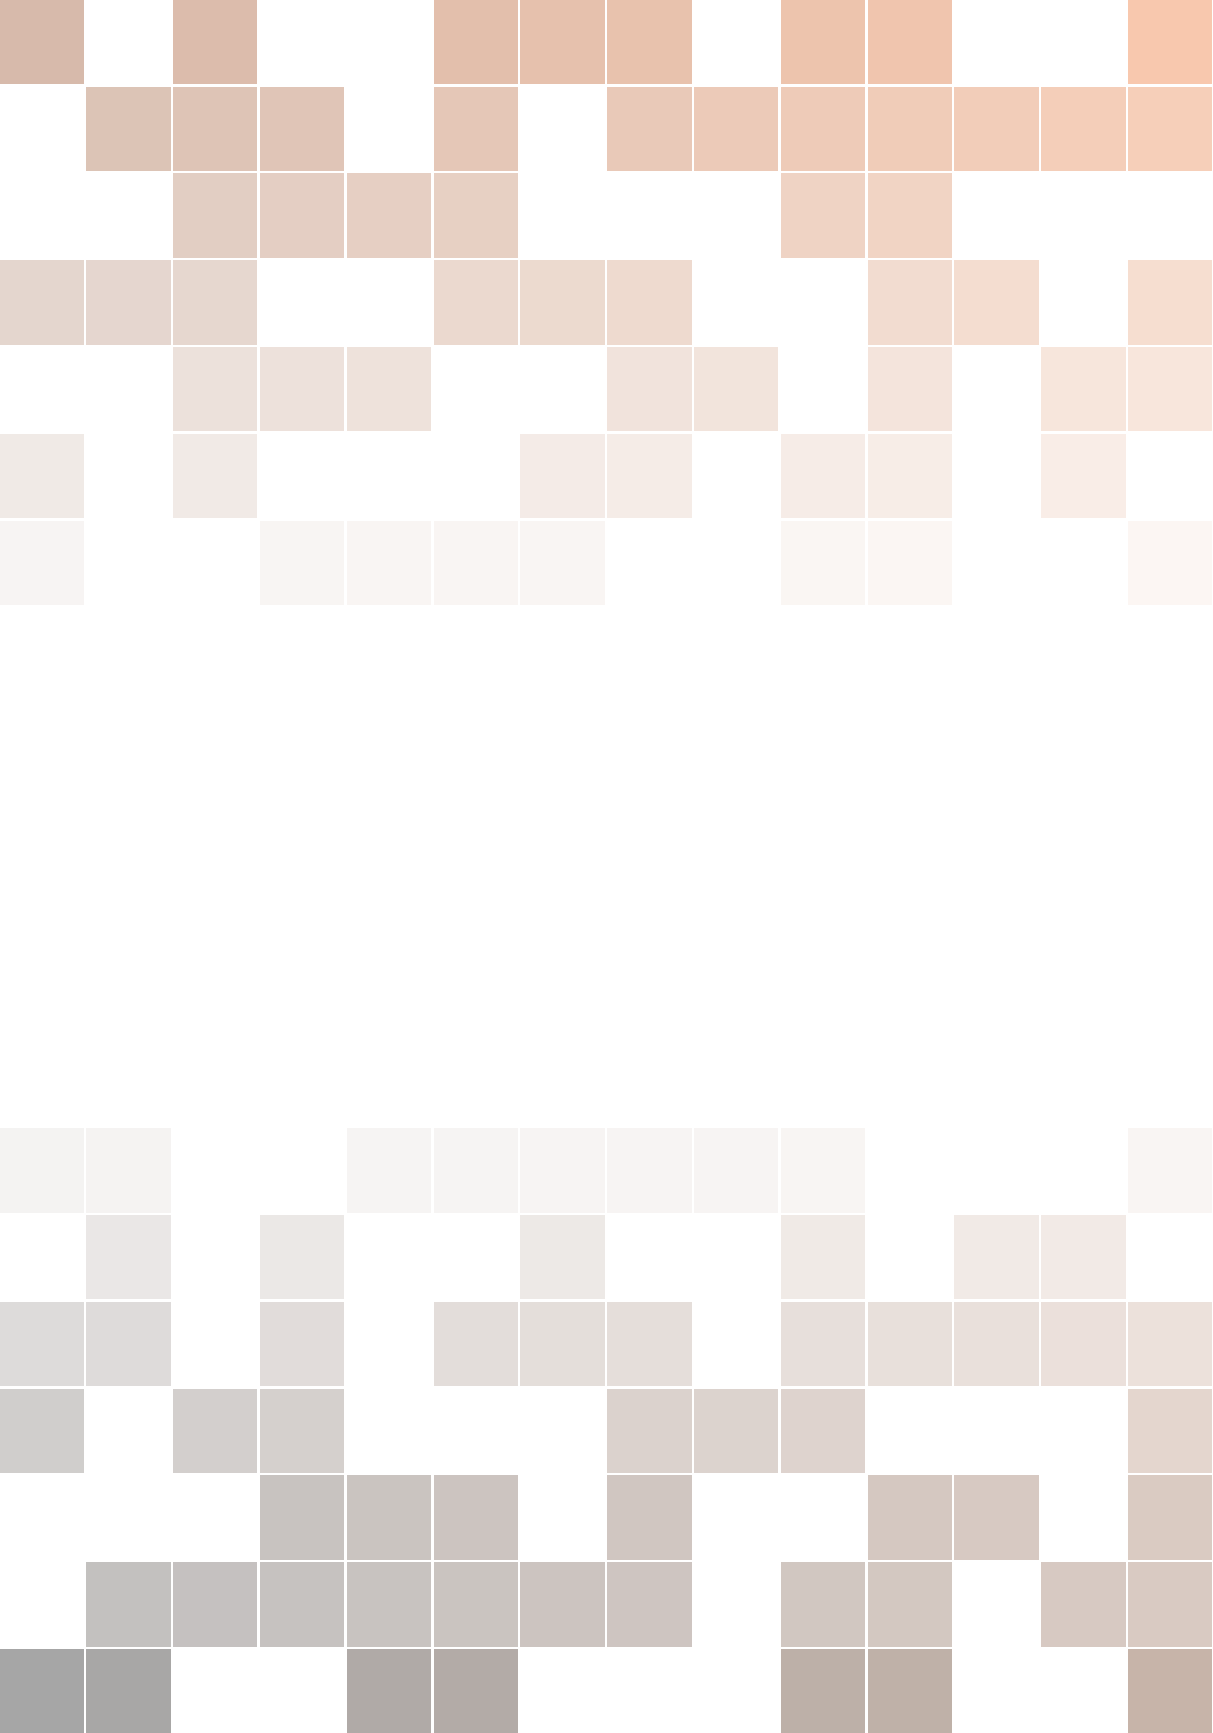
\includegraphics[scale=1]{background}}} % Image background
\centering
\vspace*{9cm}
\par\normalfont\fontsize{35}{35}\sffamily\selectfont
Representation and Reasoning for Intelligent Systems\par % Book title
\vspace*{1cm}
{\Huge Stefan Klaus}\par % Author name
\endgroup

%----------------------------------------------------------------------------------------
%	COPYRIGHT PAGE
%----------------------------------------------------------------------------------------

\newpage
~\vfill
\thispagestyle{empty}

\noindent Copyright \copyright\ Stefan Klaus\\ % Copyright notice

\noindent \textsc{NOT PUBLISHED}\\ % Publisher

\noindent \textsc{book-website.com}\\ % URL

\noindent Licensed under the Creative Commons Attribution-NonCommercial 3.0 Unported License (the ``License''). You may not use this file except in compliance with the License. You may obtain a copy of the License at \url{http://creativecommons.org/licenses/by-nc/3.0}. Unless required by applicable law or agreed to in writing, software distributed under the License is distributed on an \textsc{``as is'' basis, without warranties or conditions of any kind}, either express or implied. See the License for the specific language governing permissions and limitations under the License.\\ % License information

\noindent \textit{First printing, March 2013} % Printing/edition date

%----------------------------------------------------------------------------------------
%	TABLE OF CONTENTS
%----------------------------------------------------------------------------------------

\chapterimage{chapter_head_1.pdf} % Table of contents heading image

\pagestyle{empty} % No headers

\tableofcontents % Print the table of contents itself

\cleardoublepage % Forces the first chapter to start on an odd page so it's on the right

\pagestyle{fancy} % Print headers again

%----------------------------------------------------------------------------------------
%	CHAPTER 1
%----------------------------------------------------------------------------------------

\chapterimage{chapter_head_2.pdf} % Chapter heading image

\chapter{Chapter 1:Constraint Satisfaction Problem}


\section{Constraint Satisfaction Problem }\index{Constraint Satisfaction Problem }
Constraint satisfaction problems(CSP) are mathematical problems defined as a set of objects whose state must satisfy a number of constraints or limitations. One example of a CSP is the game “Sudoku” \\[3ex]

\section{Basic terms about CSP:}
\begin{itemize}
\item an assignment is to assign values to some or all variables
\item an assignment that does not violate any constraints is called a consistent assignment. With values from domain D\_i
\item A complete assignment is one in which each variable is assigned
\item a partial assignment is one that assigns value to some of the variables 
\end{itemize}


\textbf{Constraint graph}\\
Binary CSP: each constraint relates at most two variables, e.g: WASA
constraint graph: nodes are variables(e.g. region WA), arcs show constraints(e.g. WASA)\\[3ex]

\textbf{Varieties of Variables}\\
Discrete variables
\begin{itemize}
\item Finite Domains
\item boolean CSPs, include: boolean satisfiability(NP - complete)
\item Sudoku
\item Infinite Domains(Integers, Strings, etc.)

\item job scheduling, variables are start/end days for each job, need a constraint language, e.g. $StartJob_1$ + 5 $\leq  StarJob_3$
\end{itemize}
Continuous variables
\begin{itemize}
\item start /end times for Hubble Telescope observations
\item Unary constraints involve a single variable
\setlength{\itemindent}{3em}
\item $SA \neq Green$
\setlength{\itemindent}{0em}
\item binary constraints involve pairs of variables
\setlength{\itemindent}{3em}
\item $SA \neq WA$
\setlength{\itemindent}{0em}
\item Higher-order constraints involve 3 or more variables	
\setlength{\itemindent}{3em}
\item cryptarithmetic column constraints
\setlength{\itemindent}{0em}
\item Preferences(soft) constraints
\setlength{\itemindent}{3em}
\item red  is better than green
\item CSPs with preference are often with optimization search algorithms constraints optimization problems 
\end{itemize}


\subsection{Node Consistency}
If a node is node-consistent if all the value’s domain satisfy the variable’s unary constraints.\\[3ex]

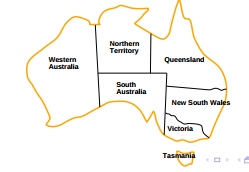
\includegraphics[scale=1]{chap1_pics/austaliaareas.png} 

Example:\\
D = {Red, Green, Blue}\\
Variable X\\
X dislikes green, then X starts with D = {Red, Green, Blue}, and becomes node consistent after eliminating {Green}.
X is node consistent with the reduced domain, D={Red, Blue}.\\

\textbf{Arc Consistency}\\
$X_i$ is arc-consistent with respect to another variables $X_j$ if for every value in $X_i$’s current domain $D_i$ there is one value in $X_i$’s domain $D_j$ that satisfies the binary constraint on the arc $(X_i , X_j)$\\[3ex]

Example:\\
Given two variables $X_i$ , $X_j$ with values in {0,1,2,...9} and constraints 
(0,0),(1,1),(2,4),(3,9).\\
To make $X_i$ arc-consistent with respect to $X_j$, we reduce $X_i$’s domain to {0,1,2,3}.\\
To make $X_j$ arc-consistent with respect to $X_i$, we reduce $X_j$’s domain to {0,1,4,9}.\\

\section{Arc Consistency Algorithm(AC-3)}
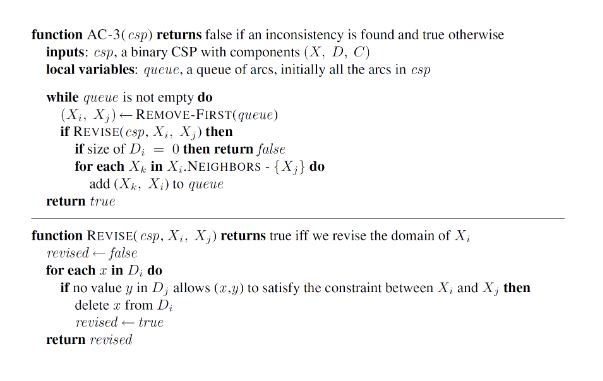
\includegraphics[scale=1]{chap1_pics/1nAyMlelLl-LW-ECO-Akl5AsNAugdRshrNF4o7Q.png} 
\begin{enumerate}
\item initially let a queue contain all arcs
\item remove an arc $(X_i , X_j)$ from the queue and make the variable $X_i$ arc-consistent to $X_j$
\begin{enumerate}
\item IF$ X_i$ domain $D_i$ is unchanged, then check the next arc in the queue
\item IF $X_i$ ‘s domain $D_i$ is revised(smaller), then add all arcs $(X_k, X_i) $in the queue 
\item If $X_i$ ’s domain $D_i$ is empty, then CSP no solution
\end{enumerate}
\item Keep checking all arcs in the queue until the queue is empty 
\end{enumerate}

\section{Path consistency}
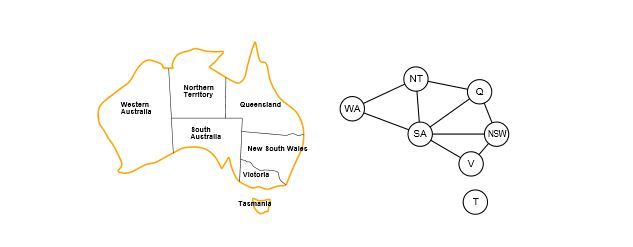
\includegraphics[scale=1]{chap1_pics/patchconsistency.jpeg} 
A two variable set ${X_i,X_j}$ is path consistency with respect to a third variable $X_m$ if for every assignment ${X_i = a, X_j = b}$ consistent with the constraints on${X_i, X_j}$, where is an assignment to $X_m$ ,that satisfies the constraints on${X_i , X_m}$ and ${X_m, X_j}$ \\[3ex]

Example:\\
Can we color the Australia map with two colors?\\
Make the set {WA, SA} path consistent with respect to NT?\\
Assignments: {WA = blue, SA = red} or {WA =blue,SA=red}\\
But no assignment exists for NT\\[3ex]

\textbf{Constraint propagation}
\begin{itemize}
\item constraint propagation is a specific type of inference 
\begin{itemize}
\item use the constraints to reduce the number of legal values for a variable, which in turn can reduce the legal values for another variable, and so on
\end{itemize}

\item node consistency
\item arc consistency
\item path consistency 
\item k-consistency: k variables involved
\item Global consistency 

\end{itemize}

\textbf{Limits}
\begin{itemize}
\item Indeed AC-3 works for the easiest Sudoku puzzles
\item slightly harder ones can be solved by PC-2, but at a greater computational cost: there are 255,960 
different path constraints to consider in a Sudoku puzzle
\item To solve the hardest puzzles and to make efficient progress, we will have to be more clever 

\end{itemize}

\section{Backtracking}
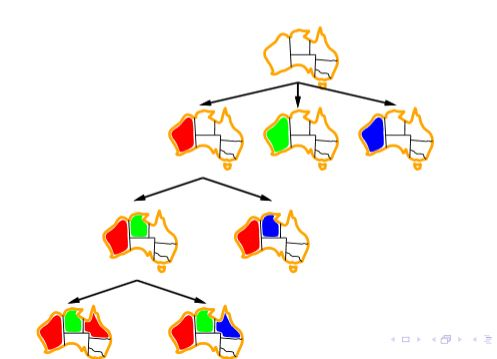
\includegraphics[scale=1]{chap1_pics/backtracking.jpeg} 

\begin{enumerate}
\item Select an unassigned value
\item assign values
\item Depth-first search
\item If an inconsistency is detected, then BACKTRACK returns failure, causing the previous call to try another value
\end{enumerate}

Backtracking search is a depth-first search for CSPs
\begin{itemize}
\item choose values for one variable at a time
\item backtrack when a variables has no legal left to assign
\end{itemize}
Backtracking search is the basic uninformed algorithm for CSP.
Can solve n-queens for $n\approx 25.$

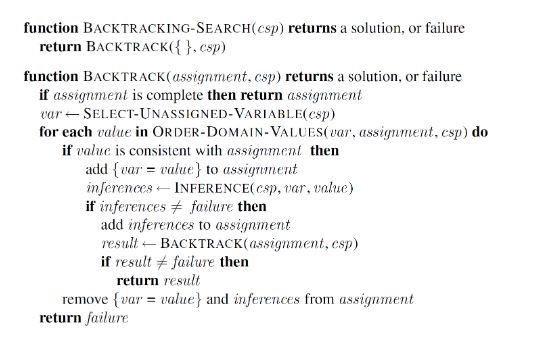
\includegraphics[scale=1]{chap1_pics/backtrackcode.jpeg}
\subsection{Improving backtracking efficiency}
General-purpose methods can give huge gains in speed:\\
\begin{enumerate}
\item which variable should be assigned next?
\item in what order should values be tried`?
\item can we detect inevitable failure early?
\item Can we take advantage of problem structure? 
\end{enumerate}

\textbf{Minimum remaining values}\\
Minimum remaining values (MRV): choose the variable with the fewest legal values.

\textbf{Degree heuristic}\\
\begin{itemize}
\item Tie-breaker among MRV variables
\item Degree heuristic: choose the variable with the most constraints on remaining variables 
\end{itemize}

\includegraphics[scale=1]{chap1_pics/backtrack2.jpeg}

\textbf{Least constraining value}\\
Given a variable, choose the least constraining value: the one that rules out the fewest values in the remaining variables.\\

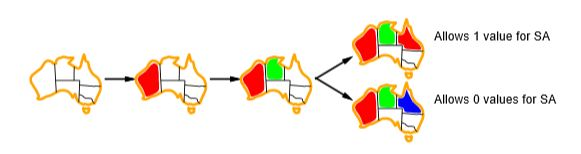
\includegraphics[scale=1]{chap1_pics/backtrack3.jpeg}
Combining these heuristics makes 1000 queens feasible.\\


\subsection{Forward checking}
Idea: Keep track if remaining legal values for unassigned variables.\\
Terminates search when any variable has no legal values.\\

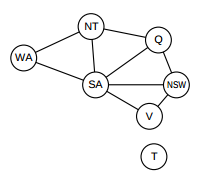
\includegraphics[scale=1]{chap1_pics/australiamap.png}\\
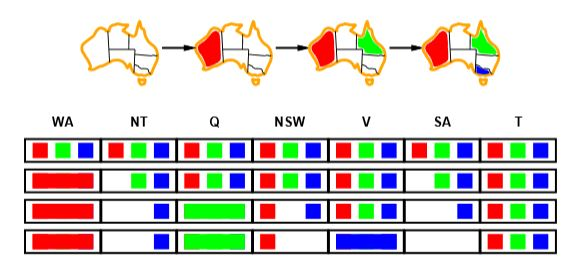
\includegraphics[scale=1]{chap1_pics/backtrack4.jpeg}

\textbf{Constraint propagation}\\
Forward checking propagates information from assigned to unassigned variables, but doesn’t provide early detection for all failures: \\
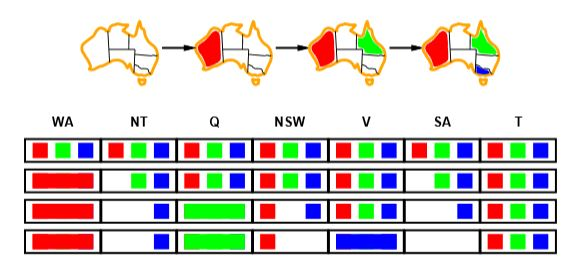
\includegraphics[scale=1]{chap1_pics/backtrack4.jpeg}

NT and SA cannot both be blue!\\
Constraint propagation repeatedly enforces constraints locally.\\

\subsection{Arc consistency}
Simplest form of propagation makes each arc consistent.\\
$X \rightarrow  Y$ is consistent if for every value x of X there is some allowed y \\[3ex]
If X looses a value, neighbours needs to be rechecked.\\
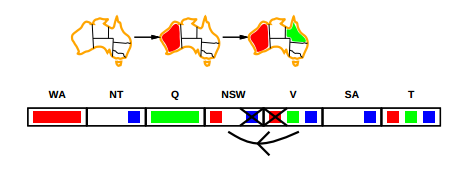
\includegraphics[scale=1]{chap1_pics/arcconsistency1.png} 

Arc consistency detects failure earlier than \textit{forward checking}.
Can be run as a predecessor or after each assignment.

\section{Structure}
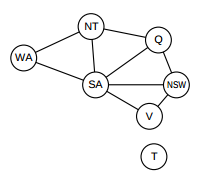
\includegraphics[scale=1]{chap1_pics/australiamap.png}\\
Tasmania and mainland Australia are independent subsections which can be identified as connected components of constraint graph. \\

\begin{itemize}
\item Suppose each subproblem has a \textit{c} variable out of \textit{n} total
\item Worst-case solution cost is $ n/c * d^c$ liniar in \textit{n}
\item E.g. $n = 80, d = 2, c =20$
\begin{itemize}
\item $2^{80}$ = 4 billion years at 10 million nodes/sec
\item $2 * 2^{20} = 0.4$ seconds at 10 million nodes/sec
\end{itemize}
\end{itemize} 

\subsection{Tree-structure CSPs}
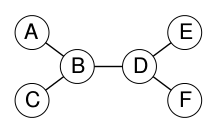
\includegraphics[scale=1]{chap1_pics/treestructure.png}

\begin{itemize}
\item Theorem: if the constraitn graph has no loops, the CSP can be solved in $O(nd^2)$ time
\item Compare to general CSPs, where worst-case time is $O(d^n)$
\item This property also applies to logical and probabilistic reasoning: an important example of the relation between syntactic restrictions and the complexity of reasoning
\end{itemize}

\subsection{Algorithm for tree-structured CSPs}
\begin{enumerate}
\item Choose a variable as root, order variables from root to leaves such that every node's parent precedes it in the ordering
\item For \textit{j} from \textit{n} down to 2, apply \textit{RemoveInconsistent}$(Parent(X_j),x_j)$
\item For \textit{j} from 1 to \textit{n}, assign $X_j$ consistently with $Parent(X_j)$
\end{enumerate}
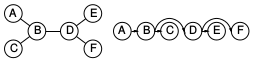
\includegraphics[scale=1]{chap1_pics/treestructurealgorithm.png} 

\subsection{Nearly tree-structured CSPs}
\begin{itemize}
\item Conditioning: instantiate a variable, prune its neighbours domains
\item Cutset conditioning: instantiate(in all ways) a set of variables such that the remaining constraint graph is a tree
\item Cutset size $c \Rightarrow runtime O(d^c * (n-c)d^2)$, very fast for small \textit{c}
\end{itemize}

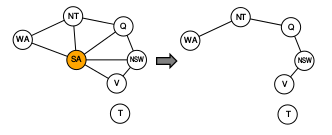
\includegraphics[scale=1]{chap1_pics/treestructuremap.png} 
\label{treestructuremap}

\begin{itemize}
\item Choose a subset \textit{S} from \textit{VARIABLE[csp]} such that the constraint graph becomes a tree after removal of \textit{S}
\item For each possible assignment to the variables in \textit{S} satisfies all constraint on S 
\begin{itemize}
\item remove from the domains of the remaining variables any values that are inconsistent with the assignment of \textit{S}
\item If the remaining CSP has solution, then return it together the assignment to S
\end{itemize}
\end{itemize}

\section{Local Search for CSPs}
\begin{itemize}
\item Local search, e.g. hill-climbing, simulated annealing for CSP
\begin{itemize}
\item typically start with a "complete" state, i.e. all variables assigned to values, but may violated constraints
\item then search changes the value of one variable at each time for violated constraints
\end{itemize}
\item Variable selection: randomly select any conflicted variable
\item Value selection by min-conflicts heuristics:
\begin{itemize}
\item choose value that violates the fewest constraints i.e. hillclimb with $h(n) = $total number of violated constraints
\end{itemize}
\end{itemize}

\subsection{Min-Conflict Algorithms}
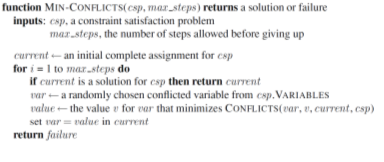
\includegraphics[scale=1]{chap1_pics/minconflictalgoithm.png} 

\begin{itemize}
\item Given random initial state, can solve \textit{n-queens} in almost constant time for arbitrary \textit{n} with high probability (e.g. $n = 10 000 000$)
\item The same to be true for any randomly-generated CSP \textit{except} in a narrow range of the ratio $R=\frac{number of constraints}{number of variables}$
\end{itemize}
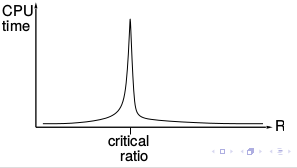
\includegraphics[scale=1]{chap1_pics/minconfliggraph.png} 



%----------------------------------------------------------------------------------------
%	CHAPTER 2
%----------------------------------------------------------------------------------------

\chapter{Chapter 2:Uncertainty}

\section{Uncertainty}\index{Uncertainty}
A purely logical approach may not work very well for statements which include multiple uncertain factors(e.g. Road accident on your way to the airport? Road work? Flooding? Nazi Zombies?\\
A purely logical approach would state: "$A_8$ will get me there on time."\\
Considering uncertain factors this would change to:"If there's no accident on the bridge, and it does not rain, and my tires remain intact etc, THEN $A_8$ will get me there on time"\\

Reasons for that:\\
\begin{itemize}
\item Failure to enumerate exceptions, qualifications etc.
\item No complete theory for the domain
\item Lack of relevant facts, initial conditions and so on
\end{itemize}

\subsection{Probability for handling uncertainty}
Probabilistic provides a way of summarizing the uncertainty.\\
An example for that would be: conditional probabilities can be used to represent:\\
\begin{itemize}
\item Given the available evidence, $A_8$ will get me there on time with probability 0.8
\item Given the available evidence, $A_10$ will get me there on time with probability 0.9
\item Given the available evidence, $A_12$ will get me there on time with probability 0.99
\end{itemize}

\begin{table}[h]
\centering
\begin{tabular}{l|l|l}
\toprule
\textbf{Condition} & \textbf{Result} & \textbf{Probability}\\
\midrule
Given the available evidence & $A_8$ & 0.9 \\
Given the available evidence & $A_10$ & 0.99\\
Given the available evidence & $A_12$ & 0.999\\
\bottomrule
\end{tabular}
\caption{Table representation of the different plans}
\end{table}

Probability theory is a main tool for dealing with degrees of belief.\\

\subsubsection{Making decisions}
Suppose given the following statements:\\

\begin{table}[h]
\centering
\begin{tabular}{l l}
P($A_8$  gets me there on time | Condition = & 0.9\\
P($A_{10}$ gets me there on time | Condition = & 0.99\\
P($A_{12}$ gets me there on time | Condition = & 0.999\\
P($A_{24}$ gets me there on time | Condition = & 0.9999\\
\end{tabular}
\end{table}

Given that, what actions to choose?\\
\begin{itemize}
\item Depends on preferences, e.g. the length of the wait at the airport
\end{itemize}

Utility theory is used to represent and infer preferences.\\
Decision theory = utility theory + probability theory\\

\section{Probability}
Subjective or Bayesian probability:\\

\begin{itemize}
\item Probabilities relate propositions to one's own state of knowledge, e.g. $P(A_8 | no reported accidents) = 0.9$
\item But might be learned from past experience from past experiences of similar situations
\item Probabilities of propositions change with new evidence: e.g. $P(A_8|no reported accidents, leave at 5 am) = 0.95$
\end{itemize}

Sample point:\\
A set $Omega $- the sample space: $\omega \in \Omega$ is a sample point or atomic event, e.g. 6 possible rolls of a dice.\\
A probability model/space is a sample space with assigning a probability for every $\omega \in \Omega$ 

\begin{itemize}
\item $P(1) = P(2) = P(3) = P(4) = P(5) = P(6) = 1/6$
\item Property: $0 \leq P(\omega) \leq 1 $ for every $\omega \in \Omega$, $\sum_{\omega \in \Omega} P(\omega) = 1$
\end{itemize}

\subsection{Event}
An event \textit{A} is any subset of $\Omega$.\\

\begin{equation}
P(A) = \sigma_{\omega \in A}P(\omega)
\end{equation}

\begin{itemize}
\item An event is 'dice roll is less than 4'
\item The probability of the event happening is $P(dice roll < 4)=P(1)+P(2)+P(3)=1/2$
\end{itemize}

In AI's language, the sets are decribed by propositions:
\begin{itemize}
\item $\phi$ is "dice roll is less than 4" 
\item $P(\phi) = \Sigma_{\omega \in \phi} P(\omega)$
\end{itemize}

\subsection{Random variables}
A random variable $X:\Omega \rightarrow R$ is a function from sample points to some range, e.g., the reals or Boolean.\\
Let $X(\omega)$ be a Boolean variable to represent whether a dicing result $\omega$ is odd, then:\\  

$X(1) = true$\\
$X(2) = False$\\

But usually written in short \textit{Odd} $P(Odd)$

\subsection{Probability Distribution}
For a random variable \textit{X} taking values from $x_1, \dots, x_k$ probability distribution $P(X = x_i)$ is the probability of \textit{X} taking the value of $x_i$:\\

\begin{table}[h]
\centering
\begin{tabular}{l l l}
$P(odd = true)$ & = & $P(1) + P(3) + P(5)$ \\
 & = & $1/6 + 1/6 + 1/6$ \\
 & = & $1/2$ \\
 $P(Odd = false)$ & = & $P(2) + P(4) + P(6)$ \\
 & = & $1/6 + 1/6 + 1/6$\\
 & = & $1/2$
\end{tabular}
\end{table}

\subsection{Prior probability}
Prior or unconditional probabilities refer to degrees of belief in propositions in the absence of any other information\\

\begin{itemize}
\item $P(Cavity = true) = 0.1$
\item $P(Weather = Sunny) = 0.72$
\end{itemize}

Probability distribution gives values for all possible probabilities:\\
$P(Weather) = <0.72, 0.1, 0.08, 0.1> $normalized, i.e. sums to 1.\\

\begin{table}[h]
\centering
\begin{tabular}{l l}
$P(Weather = sunny)$ & = 0.72\\
$P(Weather = rain)$ & = 0.1\\
$P(Weather = cloudy)$ & = 0.08\\
$P(Weather = snow)$ & = 0.1
\end{tabular}
\end{table}

\subsection{Joint Probability distribution}
Joint Probability distribution for a set of r.v.s gives the probability of every atomic event on those r.v.s(i.e. every sample point)\\

\begin{table}[h]
\centering
\begin{tabular}{|l|l|l|l|l|}
\toprule
 & \multicolumn{2}{ |c| }{Toothache} &\multicolumn{2}{ |c| }{$\neg$ Toothache}\\
 \hline
 & catch & $\neg$catch & catch & $\neq$ catch\\ 
\midrule
 cavity & 0.108 & 0.012 & 0.072 & 0.008\\
 \hline
 $\neg$cavity & 0.016 & 0.064 & 0.144 & 0.576 \\
 \bottomrule
\end{tabular}
\end{table}

\subsection{Conditional probability}
Conditional or posterior probabilities: \\
given some information, sometimes called evidence, the probability of an event happening under the evidence.

\begin{itemize}
\item If a patient is observed to have toothache and no other information is yet available, then the probability of having cavity is 0.8
\item P(cavity|tootache) = 0.8
\end{itemize}

\begin{equation}
Tootache = true \Rightarrow P(cavity|tootache) = 0.8
\end{equation}


If we know more facts e.g. cavity is also given, then we have:\\
$P(cavity|tootache, cavity) = 1$
The less specific belief \textit{remains valid} after more evidence arrives, but is not always \textit{useful}. New evidence may be irrelevant, allowing simplification, e.g.:\\
\begin{equation}
P(cavity|tootache, dice = 1) = P(cavity|tootache) = 0.8
\end{equation}


This kind of inference, sanctioned by domain knowledge, is crucial.
%----------------------------------------------------------------------------------------
%	CHAPTER 3
%----------------------------------------------------------------------------------------

\chapterimage{chapter_head_1.pdf} % Chapter heading image

\chapter{Presenting Information}

\section{Table}\index{Table}

\begin{table}[h]
\centering
\begin{tabular}{l l l}
\toprule
\textbf{Treatments} & \textbf{Response 1} & \textbf{Response 2}\\
\midrule
Treatment 1 & 0.0003262 & 0.562 \\
Treatment 2 & 0.0015681 & 0.910 \\
Treatment 3 & 0.0009271 & 0.296 \\
\bottomrule
\end{tabular}
\caption{Table caption}
\end{table}

%------------------------------------------------

\section{Figure}\index{Figure}

\begin{figure}[h]
\centering
\includegraphics[scale=0.5]{placeholder}
\caption{Figure caption}
\end{figure}


%----------------------------------------------------------------------------------------
%	CHAPTER 6
%----------------------------------------------------------------------------------------

\chapter{Chapter 7:Case-Based Reasoning}

\section{Case-Based Reasoning}\index{Case-Based Reasoning}
\begin{itemize}
\item Case law: made up of, and from, hundred and thousands of precedent cases
\item Principle: cases with similar facts should be treated in similar ways 
\item In cases where the parties disagree on what the law is: looking to past precedential decisions of relevant courts
\item If a similar dispute has been resolved in the past: following the reasoning used in the prior decision
\item If the current dispute is fundamentally distinct from all previous cases: creating new 
\item CBR: analogous to human experts solving a problem through employing their relevant past experience
\begin{itemize}
\item exemplar-based reasoning
\item instance-based reasoning
\item memory-based reasoning
\item case-based reasoning
\item analogy-based reasoning
\end{itemize}
\item if the new problem has some novel aspects, aspects, then the solution to the new problem is added to the case base
\item Different from diagnostic fault tree or rule-based system
\begin{itemize}
\item memory-based problem-solving
\item reusing past experiences
\end{itemize}
\end{itemize}

Domains that CBR Works well:
\begin{itemize}
\item Broad but shallow domain
\begin{itemize}
\item not a single tree, but a forest of small trees
\item a number of loosely connected problems that must be dealt with
\item need different kinds of expertise
\end{itemize}
\item Experience, rather than theory, is the primary source of knowledge
\begin{itemize}
\item Many past examples of problems that occur
\item rather than having a deep understanding of the domain
\end{itemize}
\item solutions are reusable
\begin{itemize}
\item old solution is useful for a new problem
\item if each problem is different, then there is little to be gained by trying to reuse past solutions
\end{itemize}
\end{itemize}

\section{Case-Based Reasoning System and 4R Cycle}
\begin{itemize}
\item Input: new problem
\item Output: a solution to the new problem
\item case base
\begin{itemize}
\item store cases(experience)
\end{itemize}
\end{itemize}

\begin{figure}[h]
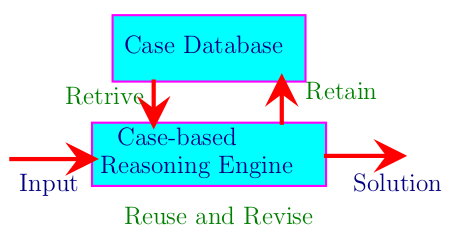
\includegraphics[scale=1]{chap7_pics/case_base_sys.png} 
\caption{The Case-Based Reasoning System}
\end{figure}


\subsection{4R Cycle}

\begin{figure}[h]
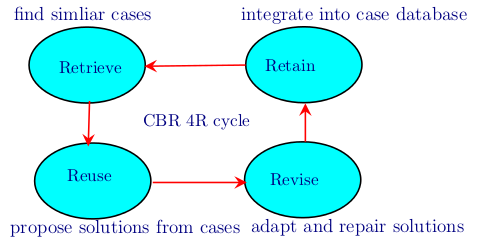
\includegraphics[scale=1]{chap7_pics/case-base-4rcycle.png} 
\caption{The Case-Based 4R cycle}
\label{case-base_4rcycle}
\end{figure}

\begin{itemize}
\item Retrieve: relevant cases, match most similar cases, retrieve solutions from theses cases
\item Reuse: solutions in stored cases
\item Revise: the retrieved solution(s) to reflect differences between new case and retrieved case(s)
\item Retain: new cases into database
\end{itemize}

See figure\ref{case-base_4rcycle} for visualisation.

\subsubsection{New Problem vs Old Case}
\begin{itemize}
\item Observations define a new problem
\item Compare similarity of each feature
\item Not all feature values may be known
\item Some features may be more important
\item New problem = case without a solution
\item Similarity by weighted average
\end{itemize}

\section{Design Case-Based Reasoning System}
\subsection{Case Representation}
A case in diagnosis represents one diagnostic situation, include two parts:\\
\begin{enumerate}
\item Features
\begin{enumerate}
\item symptoms
\item failure
\item feature values
\item repair strategies
\item test time and cost
\end{enumerate}
\item Solutions
\begin{enumerate}
\item cause of failure
\item replace or repair fault unit
\end{enumerate}
\end{enumerate}

\subsection{Design Case database}
\begin{itemize}
\item Dependent on the structure and content of its collection of cases
\begin{itemize}
\item Deciding what to store in a case
\item Finding an appropriate structure for describing case contents
\item Deciding how the case memory should be organized and indexed for effective retrieval and reuse
\end{itemize}
\end{itemize}

\subsection{Retrieve: index}
\begin{itemize}
\item Retrieve a case from case database
\item Select indexes
\begin{itemize}
\item Similar to books in library, index may help search cases in case database
\end{itemize}
\end{itemize}

\subsubsection{Match Case}
\begin{itemize}
\item Compare features and their value between the stored case and new problem
\item Nearest-neighbour matching algorithm
\end{itemize}

\subsection{Retrieval: Ranking}
\begin{itemize}
\item Possibly more than one case is matched
\item Among matched cases, ranking may be used to choose a case to reuse
\item If a matched case cannot provide the solution to the problem,. lower rank cases may be taken as the candidate for the problem
\item Ranking value will depend on observation time and cost
\begin{itemize}
\item Higher the rank $\longrightarrow$ better solution(cheaper, faster, etc.)
\item Ranking Observation cost, observation time and case frequency need to be considered
\end{itemize}
\end{itemize}

\subsection{Reuse/Revive}
\begin{itemize}
\item Adapt/repair old solutions
<<<<<<< HEAD
\end{itemize}

\subsection{Retain: Store new cases and stop reasoning}

=======
\item Different approaches
\begin{itemize}
\item Substitution
\item Parameter adjustment(via specialized heuristics, e.g. Judge)
\item Local search(replacing fruits in a recipe)
\item Special purpose adaptation and repair
\item Model-based
\end{itemize}
\end{itemize}

\subsection{Retain: Store new cases and stop reasoning}
\begin{itemize}
\item Store all new cases
\item Or store selected new cases(based on certain criteria?)
\item The reasoning stops until a satisfied solution(from a solved case) is found
\item or stop the reasoning procedure by the system
\end{itemize}
>>>>>>> 353267796def4aea94a3d8dfad13e9bdfbec6bf1


%----------------------------------------------------------------------------------------
%	BIBLIOGRAPHY
%----------------------------------------------------------------------------------------

\chapter*{Bibliography}
\addcontentsline{toc}{chapter}{\textcolor{ocre}{Bibliography}}
\section*{Books}
\addcontentsline{toc}{section}{Books}
\printbibliography[heading=bibempty,type=book]
\section*{Articles}
\addcontentsline{toc}{section}{Articles}
\printbibliography[heading=bibempty,type=article]

%----------------------------------------------------------------------------------------
%	INDEX
%----------------------------------------------------------------------------------------

\cleardoublepage
\phantomsection
\setlength{\columnsep}{0.75cm}
\addcontentsline{toc}{chapter}{\textcolor{ocre}{Index}}
\printindex

%----------------------------------------------------------------------------------------

\end{document}